\documentclass{article}%
\usepackage[T1]{fontenc}%
\usepackage[utf8]{inputenc}%
\usepackage{lmodern}%
\usepackage{textcomp}%
\usepackage{lastpage}%
\usepackage[head=40pt,margin=0.5in,bottom=0.6in]{geometry}%
\usepackage{graphicx}%
%
\title{\textbf{Indígenas en la Sierra de Perijá mueren por falta de medicinas y alimentos}}%
\author{EL NACIONAL WEB}%
\date{12/10/2018}%
%
\begin{document}%
\normalsize%
\maketitle%
\textbf{URL: }%
http://www.el{-}nacional.com/noticias/sociedad/indigenas{-}sierra{-}perija{-}mueren{-}por{-}falta{-}medicinas{-}alimentos\_255489\newline%
%
\textbf{Periodico: }%
EN, %
ID: %
255489, %
Seccion: %
Sociedad\newline%
%
\textbf{Palabras Claves: }%
Medicinas, Nutrición, Crisis humanitaria, Zulia\newline%
%
\textbf{Derecho: }%
2.9%
, Otros Derechos: %
2.10, 2.1%
, Sub Derechos: %
2.9.1, 2.10.1, 2.1.1%
\newline%
%
\textbf{EP: }%
NO\newline%
\newline%
%
\textbf{\textit{Las comunidades yukpas y barí no cuentan con acceso a los servicios básicos para combatir enfermedades como el paludismo}}%
\newline%
\newline%
%
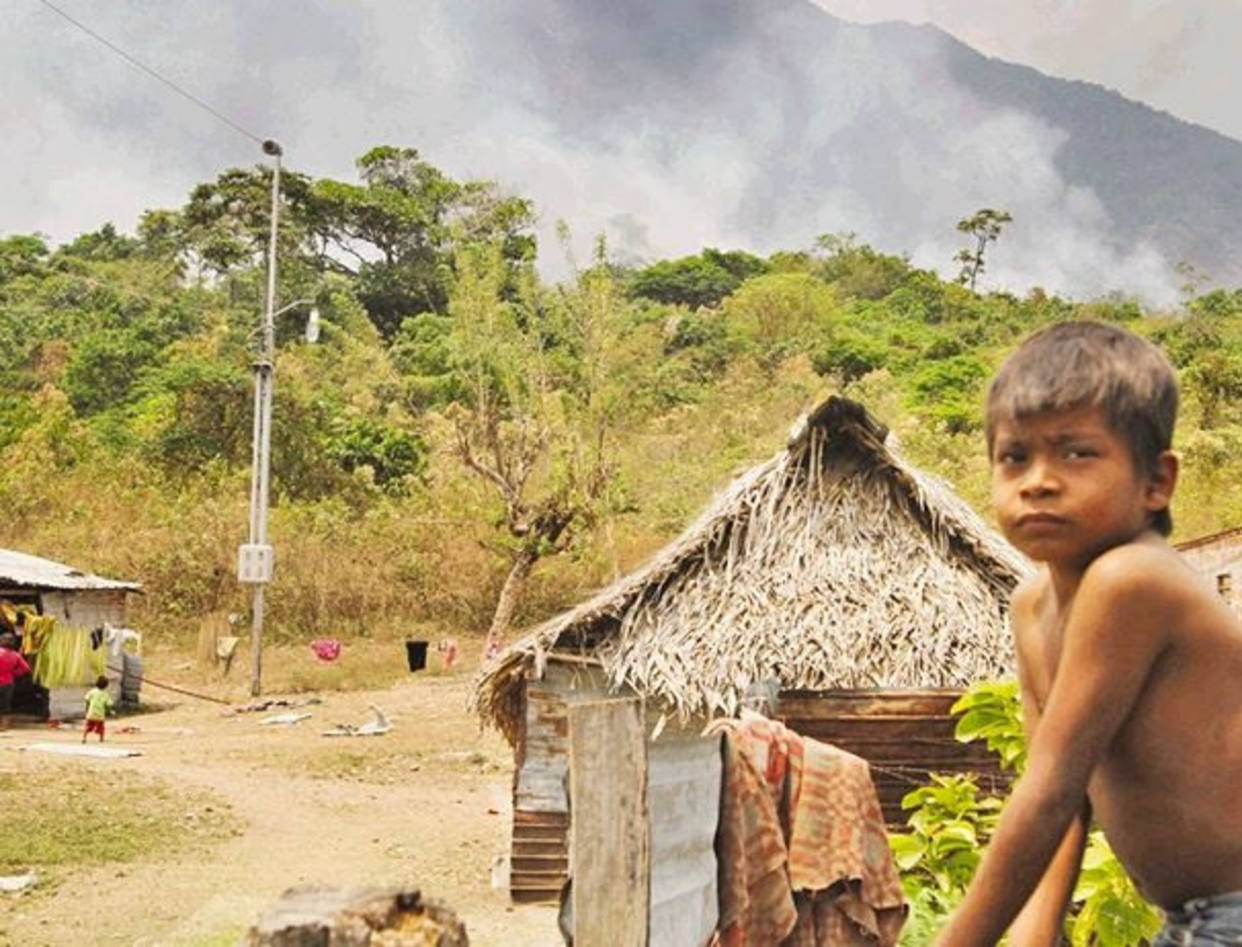
\includegraphics[width=300px]{176.jpg}%
\newline%
%
Las entidades indígenas de la Sierra de Perijá, estado Zulia, están vulnerables ante la propagación de enfermadades en el lugar debido al dificultoso acceso a medicidas y alimentos.%
\newline%
%
Los caciques de las etnias yukpas y barí denunciaron~que niños, adultos y ancianos mueren dentro de sus comunidades porque no tienen los recursos económicos para adquirir una buena alimentaciíon ni costear las medicinas para enfermedades como paludismo, diarreas y vómitos, informó~El Pitazo.%
\newline%
%
Residentes de estos grupos aborígenes alegaron que los centros de antencióm ambuatoria no cuentan con los recursos ni el personal para laborar eficientemente. "En estos momentos, las hermanas de Santa Ana son heroínas de la caridad en la atención a los enfermos de la Sierra de Perijá, a ellas se debe el ambulatorio del Tukuko, ellas lo construyeron y lo dirigieron hasta los años 80 que lo asumió el~Ministerio de Salud~y, a pesar de esto, continúan su labor de atender a los enfermos”, dijo un docente de la comunidad yukpa.%
\newline%
%
Los habitantes pueden pasar horas caminando~para llegar a una unidad médica que pueda atenderlos. Solicitaron a las autoridades que se atiendan estos casos debido a que la salud es un derecho constitucional que poseen, "no solo cuando hay elecciones" dijo un de los integrantes del grupo barí.%
\newline%
%
Propagación del paludismo%
\newline%
%
El paludismo es una de las mayores amenazas en esta~región, siendo diagnosticada en aproximadamente 100 personas en un período de cinco días. "En estos momentos no hay primaquina, el microscopio está dañado desde hace dos meses, las autoridades no nos han dado respuestas, los indígenas de la comunidad estamos recolectando dinero para ver si logramos reparar el microscopio, porque es necesario contar con ese equipo en la comunidad, las muestras se toman en el Tukuko y se llevan a la sede de malaria en Machiques" dijo Néstor Maikishi, cacique mayor de de Tukuko, subdivisión yukpa.%
\newline%
%
Estas personas tienen semanas esperando a la autoridades pertinentes del estado para que sean auxiliados con estos problemas que han afectado a más de cinco mil habitantes, dijo Maikishi.%
\newline%
%
Enfermos y mal alimentados%
\newline%
%
La desnutrición es otro tema que tiene preocupados a los encargados de estas entidades. Las familias, que suelen estar integradas por más de seis personas, comen mayormente carbohidratos que son cultivados por ellos mismos como auyama, yuca, ocumo y otras hortalizas, dejando de lados las carnes.%
\newline%
%
Maikishi destacó que tienen aproximadamente dos meses sin jornadas de alimentación en la Sierra de Perijá.~“Nuestros productos agrícolas no son suficientes para alimentarnos. También necesitamos comer pollos, huevos, harina de maíz precocida”, dijo el lídel de la etnia caribeña.%
\newline%
%
La misma comunidad realiza actividades junto a un grupo de caridad para que los niños menores de cinco años puedan ser dotados de los suplementos necesarios. Las familias acuden a estos puntos y exponen la situación de los menores.%
\newline%
%
Lea la noticia completa en~El Pitazo%
\newline%
%
\end{document}